\chapter{Mise en œuvre}
\section{La demande du client}


\section{La gestion de projet dans le projet}

\subsection{Communication au sein du projet}

Dans un projet de cette importance et mené à bien par autant de personnes, une bonne communication est essentielle afin d'éviter des situations où des personnes ne se comprennent pas au sein de l'équipe ou un rendu du projet qui ne correspond pas à l'attente du client.

Pour garantir cette bonne communication, nous avons donc organisé des réunions de groupe toutes les 2 semaines ce qui permettait de maintenir une même vision du projet, la circulation de certaines informations, ainsi que la cohésion de l'équipe.

Le groupe étant divisé en équipes de nombreuses réunions d'équipe ont aussi eu lieue, pour aider à maintenir chaque équipe dans le même objectif.

Des systèmes d'échanges d'informations ont aussi été mis en place comme le système de tickets (sur le git), afin de résoudre plus vite un problème dont quelqu'un ne trouve pas la solution seul.

De plus, la communication au sein de nôtre groupe nous a permis de définir clairement le rôle de chacun.

\subsection{Méthodologie employée}

Le développement de ce projet s'est fait selon les méthodes Extreme programming et scrum pour la plus grande partie. Ces 2 méthodes ont aidé le groupe a travailler de façon cohérente les uns par rapport aux autres.

Nous avons surtout appliqué comme principe de la méthode Extreme programming le principe d'établir les tests de façon systématique (ce qui amoindri le nombre d'erreurs à la fin du développement).

La méthode scrum s'intégrait très bien à nôtre projet, puisque ses principaux principes sont :
\begin{itemize}
\item[-] De faire en sorte que tout le monde ai une bonne vision du projet, de son avancement et de ce qu'il doit faire (y compris une personne extérieure au projet); ce que nous faisions au travers des diverses réunions de mise au point et les réunions qui visaient à mettre à niveaux des membres de l'équipe sur certains points techniques.
Maintenir cette transparence au sein du projet était aussi un des objectif formulé en cours et par le groupe.
\item[-] Le projet doit aussi être régulièrement contrôlé afin de ne pas dévier du but initial fixé par le client, ce qui cadrait avec la régularité des réunions client établie.
\item[-] Le dernier principe est de pouvoir s'adapter en cas de problème à travers des réunions d'équipes récurrentes, ce qui dans le contexte de ce projet était facilité par l'emploie du temps commun que nous avions.
\end{itemize}



Les tests étaient réalisés en amont du développement (Test Driven Development). Nous obtenions moins d'erreurs avec cette méthode.
De plus on voit clairement, une fois les tests établies à quelles exigences la fonctionnalité développée doit répondre : cela rend plus simple le développement.

\subsection{Suivie du projet}

Une bonne cohésion du groupe est essentielle (comme vu plus haut), mais on doit aussi établir une communication solide avec le client afin de répondre correctement à ses attentes.

Des réunions régulières avec les clients, qui ont eu lieu à peu près toutes les 2 semaines, ont permis de faire évoluer le projet de façon conforme, c'est à dire en accord avec les besoins des clients, jusqu'au bout du projet.

Le suivis était, pour la plus grande partie réalisé par les responsables de gestion client, qui tenaient le reste de l'équipe informé, gardant ainsi en lien bien établi avec le client.

La communication avec le client était aussi intéressante étant donné qu'il pouvait apporter des connaissances nécessaire au projet.

\subsection{Les documents de gestion de projet}

Dans un projet, les documents de gestion de projet font office de feuille de route. Ils définissent les objectifs, le cadre, les ressources humaines et les ressources en temps.

La délimitation des tâches a effectuer est donc formalisée par les différents documents de gestion de projet, ce qui nous permet un découpage efficace et donc d'avancer plus rapidement sur le développement.

Le diagramme de Gantt est un autre type de document qui est aussi d'une grande aide sur un projet comme le nôtre : on y voit clairement la situation de chacun par rapport au projet. L'avancement du projet y apparait aussi clairement de même que toute les dates importantes.
C'est un document qui avance avec l'avancement du projet et est donc très interactif.

Les documents ont donc étaient particulièrement utiles notamment l' ``analyse des risques'' dont le formalisme a rendu les sorties de ``crises'' plus simples. 
Et d'une manière plus générale, ils nous ont guidé à travers ce projet conséquent en nous évitant d'être confronté à des problèmes pour lesquels aucune solution n'était encore en place, ils nous ont aussi évité de possibles déroutes.

\subsection{Le rôle de chacun}

La définition précise du rôle de chacun permet de définir des interlocuteurs dédiés à chaque situation.
De même cela évite qu'un problème soit pris en charge par plusieurs personnes.

La composition du groupe est la suivante :
\begin{itemize}
\item Le chef d'équipe : Adrien SMONDACK (Gaëtan FERRY)
\item Les responsables de gestion client : Benjamin ZIGH et Maxime MICHOTTE
\item Le responsable qualité : Gaëtan FERRY (Claire HARDOUIN)
\item Les responsables techniques : Damien PICARD (C) Yves ADEGOLOYE (Java)
\end{itemize}

On y voit bien la situation de chaque acteur et donc à qui s'adresser selon la situation.


\subsection{La gestion de projet, conclusion}

Tout au long du projet la gestion de projet a permis une meilleure coordination au sein de l'équipe, de limiter la perte de temps dû aux digressions.

Cette approche méthodique a était bénéfique à tous les niveaux du projets (communication, prévision, développement...), elle définit un cadre nécessaire à l'accomplissement du projet.

\section{Le Module PAM}
%faire les sous sections (voir Damien)

\section{L'application Android}
\subsection{La bibliothèque de calcul}
Afin que le token soit en mesure de générer des mots de passe jetables, il était
nécessaire de développer une suite de fonctions de calcul. De plus, ces fonctions devait
être cohérentes avec celle écrites pour la vérification dans le module PAM.

La bibliothèque est découpée en trois partie distinctes tel que décrites sur la figure
\ref{fig:umlLib}. On trouve donc un ensemble de quatre classes formant la partie calcul
des mots de passe jetables, un deuxième de deux classes formant une couche d'abstraction
pour la gestion des secrets cryptographiques et enfin une dernière classe utilitaire 
contenant des fonctions nécessaires aux protocoles HOTP et TOTP.

\begin{figure}
  \centering
  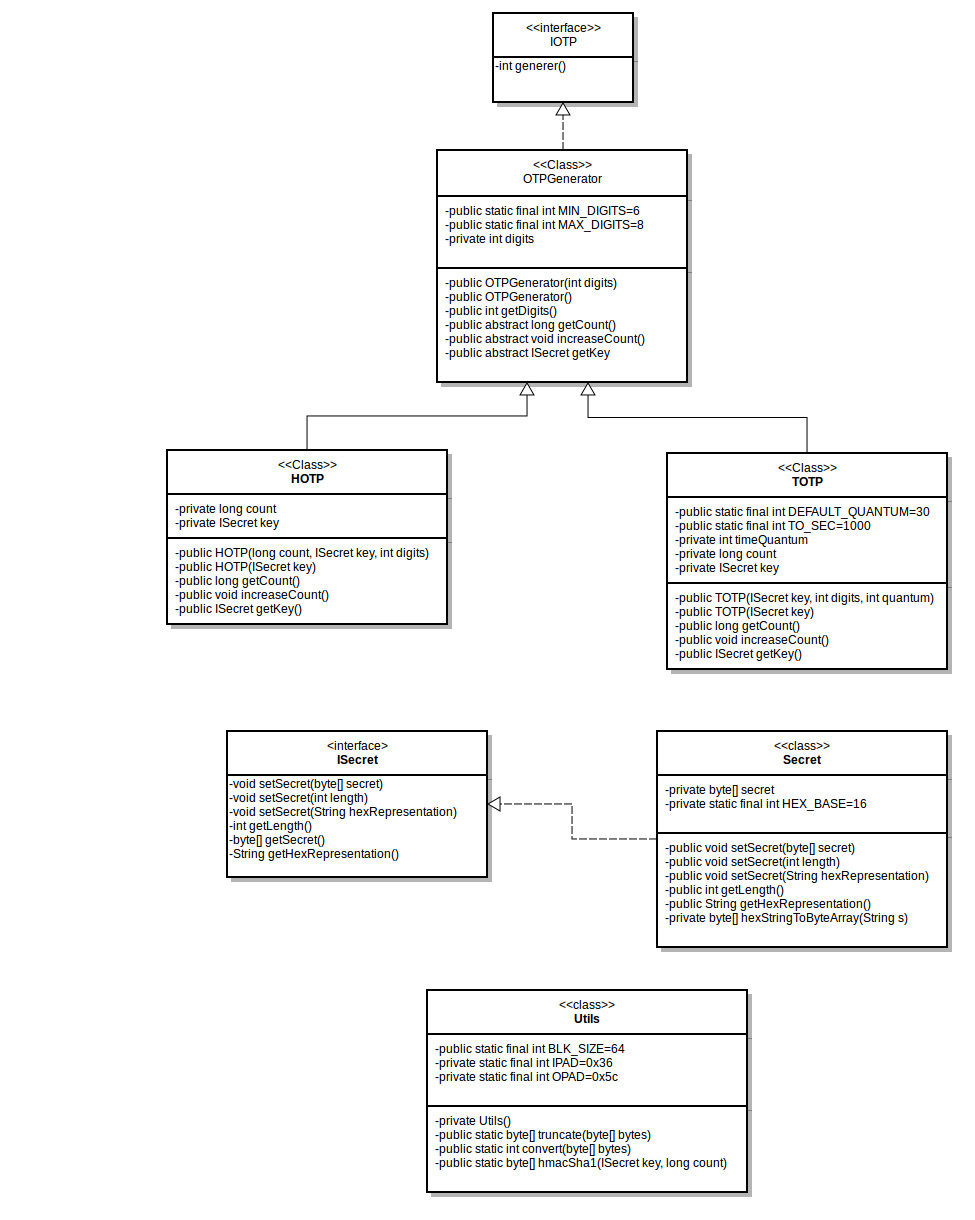
\includegraphics[scale=0.4]{../graphics/uml_lib.jpg}
  \caption{Architecture de la bibliothèque de calcul}
  \label{fig:umlLib}
\end{figure}

\subsubsection{Générateur d'OTP}
La première des trois partie définit les générateur d'OTP en eux même. Il sont répartis en
deux catégorie, correspondant aux deux méthode de génération implémentées, les générateur
TOTP et les générateur HOTP. Du fait que la spécification du protocole TOTP découle de celle
de celui d'HOTP, ces deux types d'objet sont très similaire dans leur fonctionnement. Les 
parties communes des deux classes sont donc factorisées dans une classe abstraite. On
retrouve donc explicitées dans cette classe les méthodes pour récupérer le nombre de chiffre
composant les OTP ainsi que celle pour générer ces derniers. En effet, il est possible de 
déclarer cette méthode à cette endroit en déportant la récupération du paramètre "compteur"
dans les classes inférieures. De ce fait, chacune des classes HOTP et TOTP défini sa
méthode \emph{getCounter} qui dans un cas retournera l'incrément du compteur synchronisé et 
dans l'autre la valeur $ timestamp / quantum $ définie dans la rfc 4226\cite{TOTP}. 

Le fonctionnement général des générateurs d'OTP est définit dans l'interface de
programmation IOTP. Cette interface reprend globalement le contenu des rfc 4226 et 6238.

\subsubsection{Gestion des secrets utilisateurs}
La deuxième partie formant l'abstraction des secrets cryptographiques est composée d'une 
interface de programmation, \emph{ISecret}, et d'une classe l'implémentant, \emph{Secret}.
Elle a pour but de fournir une couche d'abstraction pour simplifier l'utilisation des secrets 
qui peut s'avérer inconfortable dès lors que ces derniers mesures plusieurs dizaines de 
caractère hexadécimaux.

On pourra donc grâce à ces deux classe créer des secrets initialisable depuis des données 
binaires brutes, des représentations hexadécimales ou encore depuis des données aléatoires.
De la même manière, il sera possible de récupérer un secret sous représentation binaire ou 
sous la forme d'une chaine de caractère hexadécimaux.

\subsubsection{Fonctions utilitaires}
Enfin la dernière partie de la bibliothèque de calcul déclare des fonctions utilitaires 
nécessaires aux calculs des mots de passes jetables.


\subsection{Architecture de l'application}
\subsection{Sécurisation}
\subsection{Interface}
